\subsection{Visualization}

To visualize the results a new appearance theme is added using citygml4j. To do this the results have to be classified. For both photovoltaic and solar thermal potential three classes are defined.
\\
Photovoltaic
\begin{itemize}
\item Photovoltaic potential classes
\subitem \(>=50kWh/m^2a\), very good, color: red
\subitem \(<50kWh/m^2a\), good, color: orange
\subitem \(<30kWh/m^2a\), limited, color: yellow
\item Solar thermal potential classes
\subitem \(>=100kWh/m^2a\), very good, color: red
\subitem \(<100kWh/m^2a\), good, color: orange
\subitem \(<50kWh/m^2a\), limited, color: yellow
\end{itemize}

Due to time problems the classification is not optimal. The class boundaries are only empirical values. Furthermore the total energy output depends on the roof area. Which leads to a classification of small roofs to low class although the orientation optimal and the global radiation high. For further investigations this classification should be optimized. The Solar Atlas Berlin uses total global radiation to classify the potential, which could be used as better model.
The new appearance theme is created with citygml4j. Each roof surfaces is added as appearance member. According to the class the are linked with the corresponding diffuse color.
After writing the new CityGML file with all energy related attributes and the new appearance theme. The file is imported to a empty database. Subsequently a KML/Collada export is used to export a KML file with the new appearance IGG\_PV\_Potential. Additionally the address and the values of photovoltaic and solar thermal potential are stored in KML balloons for each building. Figure \ref{fig:vis} shows the resulting KML of the statistical block in Google Earth.

\begin{figure}[hbt!]
\centering
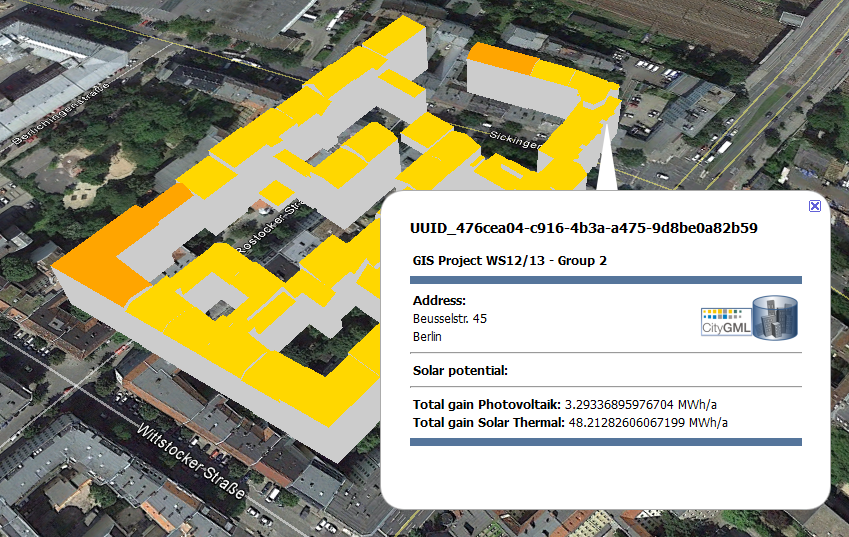
\includegraphics[width=0.7\textwidth]{phase2/group2/figure/viz.png}
\caption{KML export}
\label{fig:vis}
\end{figure}